\let\negmedspace\undefined
\let\negthickspace\undefined
\documentclass[journal]{IEEEtran}
\usepackage[a5paper, margin=10mm, onecolumn]{geometry}
\usepackage{lmodern} % Ensure lmodern is loaded for pdflatex
\usepackage{tfrupee} % Include tfrupee package

\setlength{\headheight}{1cm} % Set the height of the header box
\setlength{\headsep}{0mm}     % Set the distance between the header box and the top of the text

\usepackage{gvv-book}
\usepackage{gvv}
\usepackage{cite}
\usepackage{amsmath,amssymb,amsfonts,amsthm}
\usepackage{algorithmic}
\usepackage{graphicx}
\usepackage{textcomp}
\usepackage{xcolor}
\usepackage{txfonts}
\usepackage{listings}
\usepackage{enumitem}
\usepackage{mathtools}
\usepackage{gensymb}
\usepackage{comment}
\usepackage[breaklinks=true]{hyperref}
\usepackage{tkz-euclide} 
\usepackage{listings}                                      
\def\inputGnumericTable{}                                 
\usepackage[latin1]{inputenc}                                
\usepackage{color}                                            
\usepackage{array}                                            
\usepackage{longtable}
\usepackage{multicol}
\usepackage{calc}                                             
\usepackage{multirow}                                         
\usepackage{hhline}                                           
\usepackage{ifthen}                                           
\usepackage{lscape}
\begin{document}

\bibliographystyle{IEEEtran}
\vspace{3cm}

\title{9.1.7}
\author{EE24BTECH11006 - Arnav Mahishi}
% \maketitle
% \newpage
% \bigskip
{\let\newpage\relax\maketitle}

\renewcommand{\thefigure}{\theenumi}
\renewcommand{\thetable}{\theenumi}
\setlength{\intextsep}{10pt} % Space between text and floats


\numberwithin{equation}{enumi}
\numberwithin{figure}{enumi}
\renewcommand{\thetable}{\theenumi}


\textbf{Question}:\newline
Solve the differential equation $y^{\prime\prime\prime}+2y^{\prime\prime}+y^{\prime} = 0$ with initial conditions $y\brak{0} = 1$,$y^{\prime}\brak{0} = -1$ , and $y^{\prime\prime}\brak{0} = 1$
\newline
\textbf{Solution: }
\begin{table}[h!]    
  \centering
  \begin{tabular}{|l|l|l|}
\hline
\textbf{Component} & \textbf{Arduino Pin} & \textbf{Description} \\
\hline
\multicolumn{3}{|c|}{\textbf{LCD Display}} \\
\hline
RS & PB0 (Digital 8) & Register Select line \\
\hline
E & PB1 (Digital 9) & Enable line \\
\hline
D4 & PB2 (Digital 10) & Data line 4 \\
\hline
D5 & PB3 (Digital 11) & Data line 5 \\
\hline
D6 & PB4 (Digital 12) & Data line 6 \\
\hline
D7 & PB5 (Digital 13) & Data line 7 \\
\hline
\multicolumn{3}{|c|}{\textbf{7-Segment Display}} \\
\hline
Segment A & PD4 (Digital 4) & Segment A line \\
\hline
Segment B & PD5 (Digital 5) & Segment B line \\
\hline
Segment C & PD6 (Digital 6) & Segment C line \\
\hline
Segment D & PD7 (Digital 7) & Segment D line \\
\hline
Common HH\_1 & PC0 (Analog 0) & Hours tens digit common \\
\hline
Common HH\_2 & PC1 (Analog 1) & Hours ones digit common \\
\hline
Common MM\_1 & PC2 (Analog 2) & Minutes tens digit common \\
\hline
Common MM\_2 & PC3 (Analog 3) & Minutes ones digit common \\
\hline
Common SS\_1 & PC4 (Analog 4) & Seconds tens digit common \\
\hline
Common SS\_2 & PC5 (Analog 5) & Seconds ones digit common \\
\hline
\multicolumn{3}{|c|}{\textbf{Buttons}} \\
\hline
Toggle Button & PD2 (Digital 2) & For cycling through options \\
\hline
Select Button & PD3 (Digital 3) & For selecting options \\
\hline
\end{tabular}
  \caption{Variables Used}
  \label{tab1.1.2.2}
\end{table}
\newline
Theoretical Solution:
We apply the Laplace transform to each term in the equation. The Laplace transforms for the derivatives of $y\brak{t}$ are:
\begin{align}
\mathcal{L}\fbrak{y^{\prime}\brak{t}} &= sY\brak{s} - y\brak{0} \\
\mathcal{L}\fbrak{y^{\prime\prime}\brak{t}} &= s^2Y\brak{s} - sy\brak{0} - y^{\prime}\brak{0} \\
\mathcal{L}\fbrak{y^{\prime\prime\prime}\brak{t}} &= s^3Y\brak{s} - s^2 y\brak{0} - sy^{\prime}\brak{0} - y^{\prime\prime}\brak{0}
\end{align}
Now, applying the Laplace transform to the entire differential equation:
\begin{align}
\mathcal{L}\{y^{\prime\prime\prime} + 2y^{\prime\prime} + y^{\prime}\} = 0\\
\mathcal{L}\{y^{\prime\prime\prime}\brak{t}\} + 2\mathcal{L}\{y^{\prime\prime}\brak{t}\} + \mathcal{L}\{y^{\prime}\brak{t}\} = 0 \\
(s^3 Y\brak{s} - s^2 y\brak{0} - s y^{\prime}\brak{0} - y^{\prime\prime}\brak{0}) + 2(s^2 Y\brak{s} - s y\brak{0} - y^{\prime}\brak{0}) + (s Y\brak{s} - y\brak{0}) = 0
\end{align}
Substitute the initial conditions $y\brak{0} = 1$, $y^{\prime}\brak{0} = -1$, and $y^{\prime\prime}\brak{0} = 1$:
\begin{align}
\brak{s^3 Y\brak{s} - s^2 \cdot 1 - s \cdot (-1) - 1} + 2\brak{s^2 Y\brak{s} - s \cdot 1 - (-1)} + \brak{s Y\brak{s} - 1} &= 0 \\
s^3 Y\brak{s} - s^2 + s - 1 + 2s^2 Y\brak{s} - 2s + 2 + s Y\brak{s} - 1 &= 0
\end{align}

Simplify the equation:
\begin{align}
&(s^3 + 2s^2 + s) Y\brak{s} - (s^2 - s + 1) - (2s - 2) - 1 &= 0 \\
&(s^3 + 2s^2 + s) Y\brak{s} - s^2 - s + 1 - 2s + 2 - 1 &= 0 \\
&(s^3 + 2s^2 + s) Y\brak{s} - (s^2 + s) &= 0
\end{align}
Now, solve for \( Y\brak{s} \):
\begin{align}
\brak{s^3 + 2s^2 + s} Y\brak{s} &= s^2 + s \\
Y\brak{s} &= \frac{s^2 + s}{s(s+1)^2}\\
\implies Y\brak{s} &= \frac{1}{s + 1}
\end{align}
Now, take the inverse Laplace transform:
\begin{align}
\mathcal{L}^{-1}\brak{\frac{1}{s + 1}} = e^{-t}u\brak{t}
\end{align}
Thus, the solution to the differential equation is:
\begin{align}
   y\brak{t} = e^{-t}u\brak{t}
\end{align}
\newline
Radius of Convergence:\\
The denominator indicates a pole at $s=-1$.To ensure convergence of the Laplace transform integral, the real part of $s$ must satsify:
\begin{align}
    Re\brak{s}>-1
\end{align}
Since the ROC extends infinitely to the right in the s-plane, the radius of convergence is:
\begin{align}
    R=\infty
\end{align}
Computational Solution:\\
Consider the given linear differential equation
\begin{align}
	a_{n}y_{n} + a_{n-1}y_{n-1} + \dots + a_{1}y_1 + a_{0}y_{0} + c = 0
\end{align}
Where $y_{i}$ is the $i$th derivative of the function then
\begin{align}
    \myvec{y_{0}^{\prime}\\y_{1}^{\prime}\\y_{2}^{\prime}\\ \vdots\\y^{\prime}_{n-1}}&=\myvec{y_{1}\\y_{2}\\y_{3}\\ \vdots\\ \frac{-\brak{\sum_{i=0}^{i=n-1}a_iy_i}-c}{a_n}}\\
    \implies  \myvec{1\\y_{0}^{\prime}\\y_{1}^{\prime}\\y_{2}^{\prime}\\ \vdots\\y^{\prime}_{n-1}}&=\myvec{1&0&0&\cdots&\cdots&\cdots&\cdots\\0&0&1&0&\cdots&\cdots&\cdots\\0&0&0&1&0&\cdots&\cdots\\0&0&0&0&1&0&\cdots\\ \vdots&\vdots&\vdots&\vdots&\vdots&\vdots&\ddots\\ \frac{-c}{a_n}&\frac{-a_{0}}{a_n}&\frac{-a_{1}}{a_n}&\frac{-a_{2}}{a_n}&\cdots&\cdots&\frac{-a_{n-1}}{a_n}}\myvec{1\\y_{0}\\y_{1}\\y_{2}\\ \vdots\\y_{n-1}}\\
    \implies \vec{y}_k^{\prime}&=A\vec{y}_k
\end{align}
Where $\vec{y}_k$ is the vector $\myvec{1\\y_{0,k}\\y_{1,k}\\y_{2,k}\\ \vdots\\y_{n-1,k}}$ at a $k$.\\
Using the trapezoidal rule,
\begin{align}
    J &= \int_a^b f\brak{x}\, dx\\
    &\approx h\brak{\frac{1}{2}f\brak{x} + f\brak{x_1} + f\brak{x_2} \cdots + f\brak{x_{n-1}} + \frac{1}{2}f\brak{b}}\\
    \frac{\vec{y}_{n+1} - \vec{y}_n}{1}\brak{\frac{1}{2} + \frac{1}{2}}
    &= A\frac{x_{n+1} - x_{n}}{1}\brak{\frac{\vec{y}_n}{2} +\frac{\vec{y}_{n+1}}{2}} \\ 
    \xrightarrow{} \vec{y}_{k+1}&=\brak{I-\frac{h}{2}A}^{-1}\cdot\brak{I+\frac{h}{2}A}\cdot\vec{y}_k
\end{align}
Bilinear Transform:\\
Another way we can arrive at the difference equation is by using the Bilinear transform, applying Laplace transform to both sides of the differential equation,
\begin{align}
    s^3 Y\brak{s} - s^2 + s - 1 + 2s^2 Y\brak{s} - 2s + 2 + s Y\brak{s} - 1 &= 0\\
    (s^3 + 2s^2 + s) Y\brak{s} - (s^2 + s) &= 0\\
    \brak{s^3 + 2s^2 + s} Y\brak{s} &= s^2 + s \\
Y\brak{s} &= \frac{s^2 + s}{s(s+1)^2}\\
\implies Y\brak{s} &= \frac{1}{s + 1}
\end{align}
Apply Bilinear Transform with $T=h$
\begin{align}
    s&=\frac{2}{T}\frac{1-z^{-1}}{1+z^{-1}}\\
    Y\brak{z}&=\frac{1}{\frac{2}{T}\cdot\frac{1-z^{-1}}{1+z^{-1}}+1}\\
    Y\brak{z}&=\frac{1+z^{-1}}{\frac{2}{h}\brak{1-z^{-1}}+\brak{1+z^{-1}}}\\
    \implies Y\brak{z}&=\frac{1+z^{-1}}{\brak{1+\frac{2}{h}}-\brak{1-\frac{2}{h}}z^{-1}}\\
    \implies \text{Taking }\alpha&=\frac{1-\frac{2}{h}}{1+\frac{2}{h}}\\
    \implies Y\brak{z}&=\frac{\brak{1-\alpha}\brak{1+z^{-1}}}{2\brak{1+\alpha z^{-1}}}\\
    \brak{1+\alpha z^{-1}}Y\brak{z}&=\frac{1-\alpha}{2}\brak{1+z^{-1}}\\
\end{align}
Applying Inverse Z transform, we get the following difference equation
\begin{align}
    y_n&=\frac{1-\alpha}{2}\brak{1+y_{n-1}}\\
    \implies y_n&=\frac{2}{1-\alpha}\delta\brak{n}+\frac{2}{1-3\alpha}y_{n-1},\abs{\alpha}<1
\end{align}
Trapzoidal form:\\
Using trapezoidal form when $h$ is the step-size For the system $\vec{y}^\prime=A\vec{y}$, the equation gives:
\begin{align}
    \frac{\vec{y}_{k+1}-\vec{y}_k}{h}=A\cdot\frac{\vec{y}_{k+1}+\vec{y}_{k}}{2}
\end{align}
Rearranging:
\begin{align}
    \vec{y}_{k+1}=\brak{I-\frac{h}{2}A}^{-1}\cdot\brak{I+\frac{h}{2}A}\cdot\vec{y}_k
\end{align}
For any particular differential equation derive $B_1$ and $B_2$ to find $\vec{y}_{k+1}$ from $\vec{y}_k$
\begin{align}
    B_1=\brak{I-\frac{h}{2}A}\\
    B_2=\brak{I+\frac{h}{2}A}
\end{align}
For $y^{\prime\prime\prime}+2y^{\prime\prime}+y^{\prime} = 0$ we get
\begin{align}
    A&=\myvec{0&1&0\\0&0&1\\0&-1&-2}\\
    \implies B_1&=\myvec{1&\frac{-h}{2}&0\\0&1&\frac{-h}{2}\\0&\frac{h}{2}&1+h}\\
    \implies B_2&=\myvec{1&\frac{h}{2}&0\\0&1&\frac{h}{2}\\0&\frac{-h}{2}&1-h}\\
\end{align}
When $k$ ranges from $0$ to $\frac{t_o-t_f}{h}$ in increments of $1$, discretizing the steps gives us all $\vec{y}_k$, Record the $y_{0,k}$ for each $k$ we got and then plot the graph. The result will be as given below.As we can see from the two graphs below the graph for bilnear transform is more accurate than the one found by finite differences proving its superiority.
\begin{figure}[H]
   \centering
   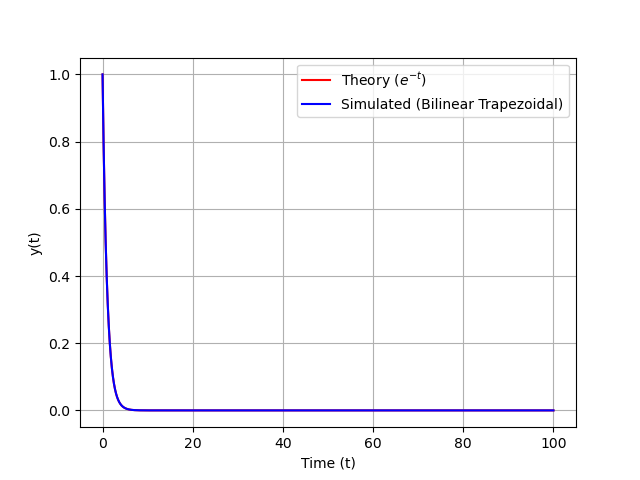
\includegraphics[width=1\linewidth]{figs/fig.png}
   \caption{Comparison between the Theoretical solution and Computational solution for Bilinear Transform}
   \label{stemplot}
  \end{figure}
 \begin{figure}[H]
 \centering
   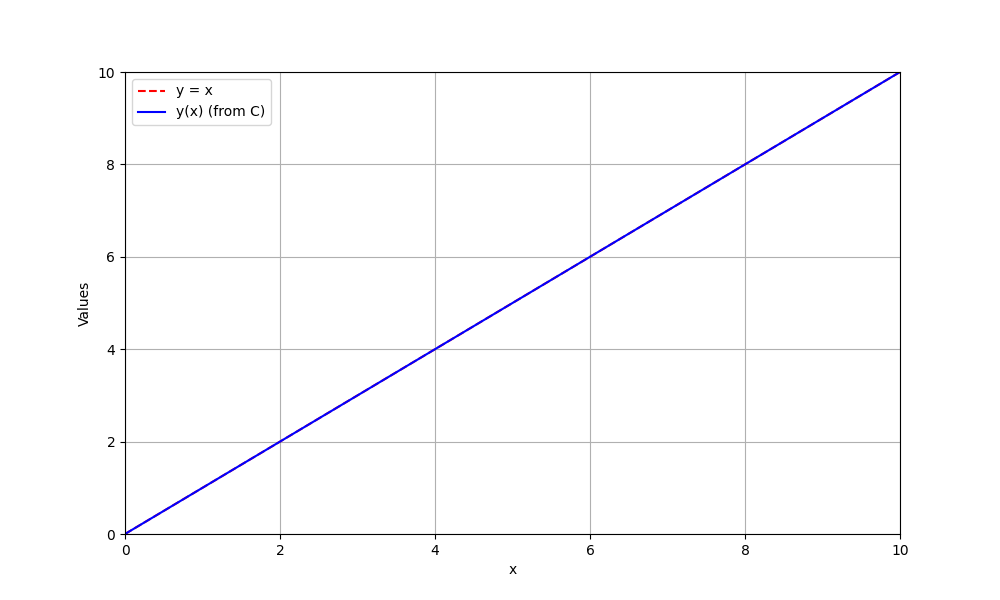
\includegraphics[width=1\linewidth]{../Problem 1/figs/fig.png}
   \caption{Comparison between the Theoretical solution and Computational solution for Finite Differences}
\end{figure}
\end{document}
